\scanpage{391}
\mspage{198}
se remonte de façon unique en
$\widehat{\widehat{\mathcal G}}^{G}$.
Il faudrait réexaminer ceci de façon plus soigneuse par la suite.
Mais il me semble qu'on ne trouve pas ici de nouvelles propriétés des
$\Gamma\subset\mathcal M_a$ ou de
$M_a$ lui $\overline{\mathrm m}$, i.e. de
$\mathbb{\Gamma}_a$ comme ss-groupe profini de
$\Gamma'=\operatorname{Norm}_{\widehat{\widehat{\mathcal T}}}
(\widehat{\mathcal T})/\widehat{\mathcal T}$.

\uline{31}\quad Digression sur les relèvements
d'\inserted{une} action extérieure
d\deleted{\unsure{e}}\inserted{'un} groupe fini $G$ sur un
groupe profini à lacets $\pi$.
\figure{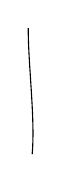
\begin{tikzpicture}[x=1cm,y=1cm,baseline=(current bounding box.south)]
\draw[line width=0.4pt] (0,0) .. controls (0.04,0.45) and (-0.05,1.12) .. (-0.05,1.60);
\end{tikzpicture}}

On suppose l'action extérieure \uline{fidèle},
i.e. $G\subset\widehat{\widehat{\mathcal T}}(\pi)
=\widehat{\widehat{\mathcal T}}$,
\inserted{et que $G=G^+$.}
On suppose de plus qu'il existe une discrétification
invariante $\pi_0$, i.e. telle que
$G\subset\mathcal T(\pi_0)$.

Si on suppose $G$ cyclique, alors sauf
erreur il est prouvé que la situation est
\uline{réalisable} topologiquement (\unsure{donc} :
\uline{\unsure{algébr.}} de façon analytique complexe $\ldots$).

\scanpage{392}
Dans le cas discret, la signification des classes de
\inserted{$\pi_0$-}conjugaison de relèvement
$G\longrightarrow\mathcal G(\pi_0)$ est bien comprise ;
\deleted{Mais}\inserted{de $\overline{\mathrm m}$ que pour les relèvements partiels}
On trouve une \deleted{\unsure{cat.} $U^{!}$} réalisation
\inserted{canonique} du groupoïde fondamental
\margin{si $U^{!}\ne\unsure{\varnothing|\phi}$}
associé au
groupe ext. $\pi_0$, par un groupoïde \inserted{fini} $[U^{!}]$
sur lequel $G$ opère au sens strict, dont les pts
correspondent aux classes de $\pi_0$-conjugaison de sections
partielles $\ne1$ maximales, le groupe
\deleted{\illegible{1}}$\mathcal T(\pi_0)^G$
opère de façon \unsure{également} canonique sur ce groupoïde.
Si $P\in U^{!}$ correspond à un relèvement
$G\longrightarrow\mathcal G(\pi_0)$, alors
un élément $\deleted{\unsure{g}}\inserted{\dot u}\in
\mathcal T(\pi_0)^G$ est dans l'image de
$\mathcal G(\pi_0)^G$, i.e. peut se remonter en
$u\in\mathcal G(\pi_0)$ commutant à $G$, sss
$\dot u(P)=P$ [i.e. sss
\inserted{(si $\dot u$ est remonté de façon \unsure{quelc.} en $v$)}
$v(G)$ est $\pi_0$-conjugué à $G$
i.e. sss $\exists g\in\pi_0$ tel que
$v(G)=\operatorname{int}(g)(G)$
i.e. \deleted{\unsure{qui}}
$u\overset{\text{déf}}{=}\operatorname{int}(g^{-1})v$ fixe $G$.
\deleted{\unsure{(Donc}} (auquel cas bien sûr il centralise,
\inserted{(par l'hyp. $\dot u\in\mathcal T^{G}$)})
Donc notre brillante assertion, est une tautologie]

\scanpage{393}
\mspage{199}
et donc le relèvement est unique. Comme
$U^{!}_{\unsure{*|\varphi}}$ est fini, donc le stabilisateur
$\mathcal T(\pi_0)^G_P$ de $P$ dans
$\mathcal T(\pi_0)^G$ est d'indice fini,
et c'est donc ce ss-groupe d'indice fini qui se remonte
gaillardement et canoniquement.

Que peut-on dire dans le contexte profini ? Bien sur,
on a une application canonique
\diagram{\begin{tikzcd}[ampersand replacement=\&,column sep=large]
\begin{gathered}
\text{\deleted{\unsure{Ens.}} classes de $\pi_0$-conj.}\\
\text{de relèvements de}\\
G\text{ en }G
\longrightarrow\mathcal G(\pi_0)\\
\text{i.e. de scindages de}\\
\text{l'ext. }1\longrightarrow\pi_0\longrightarrow
E\longrightarrow G\longrightarrow1
\end{gathered}
\arrow[r] \&
\begin{gathered}
\text{classes de $\pi_0$-}\\
\text{conj. de rel. de}\\
G\text{ en }G
\longrightarrow\widehat{\widehat{\mathcal G}}(\pi_0)\\
\text{i.e. de scindages}\\
\text{de l'extension}\\
1\longrightarrow\underset{\substack{\Vert\\\pi}}{\widehat{\pi}_0}
\longrightarrow\widehat E
\longrightarrow G\longrightarrow1
\end{gathered}
\end{tikzcd}}

Il faudrait examiner d'abord

a) La question de la bijectivité de cette appl.

b) La question si $\pi^G=1$ (\unsure{\uline{rigidité}|rigidité}),
pour $G\ne(1)$. -- (pour un relèvement donné,
dans $E$ pour simplifier)

J'ai envie de conjecturer sans vergogne
qu'il en est ainsi --- ce qui impliquerait
p.ex. que pour tt tel relèvement $G$, il y a

\scanpage{394}

un sous-groupe \uline{ouvert} \inserted{$(\unsure{\widehat{\widehat{\mathcal T}}|\widehat{\mathcal T}}^{G})_{P}$} du groupe (peut-être vraiment immense à priori !) $\widehat{\widehat{\mathcal T}}^{G}$, qui se remonte canoniquement de façon à commuter à \unsure{$\widetilde G$|$G$}....

Il faudrait manifestement faire, en $\overline{\mathrm m}$ temps qu'une théorie des op. ext. de groupes finis sur des groupes discrets à lacets (qui est pour le moment extrêmement \unsure{conjecturale|conjectural}) une théorie analogue dans le cas profini --- j'\deleted{\illegible{1}}\inserted{aurai} sans doute à y revenir par la suite.

\scanpage{395}
\mspage{200}

\uline{32} Retour sur les aspects arithmétiques du bouchage de trous : relations entre $\Gamma_{g,\nu}$ et $\Gamma_{g,\nu-1}$.

Bien sûr, on \deleted{\unsure{voit que}} a que
\[
\mathcal N_{g,\nu}\longrightarrow\mathfrak S_{\nu}
\]
est surjectif \inserted{(puisque $\mathcal T_{g,\nu}\longrightarrow\mathfrak S_{\nu}$ l'est)}, donc on aura
\[
(1)\qquad 1\unsure{\longrightarrow|-}\mathcal N_{g,\nu}^{!}\unsure{\longrightarrow|-}\mathcal N_{g,\nu}\unsure{\longrightarrow|-}\mathfrak S_{\nu}\unsure{\longrightarrow|-}1
\]
et le diagramme cartésien de \unsure{ssgroupes} de $\widehat{\widehat{\mathcal T}}_{g,\nu}$
\[
(2)\qquad
\diagram{\begin{tikzcd}[ampersand replacement=\&]
\widehat{\mathcal T}_{g,\nu}^{+}\arrow[r,hook] \& \mathcal N_{g,\nu}\\
\widehat{\mathcal T}_{g,\nu}^{!+}\arrow[u,hook]\arrow[r,hook] \& \mathcal N_{g,\nu}^{!}\arrow[u,hook]
\end{tikzcd}}
\]
\margin{\deleted{\illegible{1}} $\mathcal N_{g,\nu}=\mathcal N_{g,\nu}^{!}\cdot\widehat{\mathcal T}_{g,\nu}^{+}$ i.e. $\mathcal N_{g,\nu}$ connu par $\mathcal N_{g,\nu}^{!}$}
donnera un isomorphisme
\[
(3)\qquad \mathcal N_{g,\nu}^{!}/\widehat{\mathcal T}_{g,\nu}^{!+}\xrightarrow{\sim}\mathcal N_{g,\nu}/\widehat{\mathcal T}_{g,\nu}^{+}=\mathbb{\Gamma}_{g,\nu}
\]
Dans le cas d'un $(\pi,a)$, \inserted{($\pi$ groupe ext. à lacets,} $a$ une arithmétisation), on aura de $\overline{\mathrm m}$
\[
(4)\qquad\left\{\begin{aligned}
\mathcal N_a^{!}/\widehat{\mathcal T}_a^{+}&\simeq\mathcal N_a/\widehat{\mathcal T}_a^{+}=\mathbb{\Gamma}_a.\\
\mathcal N_a&=\mathcal N_a^{!}\widehat{\mathcal T}_a^{+}
\end{aligned}\right.
\]

Considérons maintenant \deleted{une \unsure{partie}\inserted{\unsure{$i\in I=I(\pi)$}} , \illegible{3} $\unsure{(g,\nu)}$, \unsure{et un} $\pi_i'$ \illegible{2} $\unsure{I=I(\pi)}$, et soit \illegible{1}} pour $\forall i\in I$ le stabilisateur \deleted{\illegible{1}} $\mathcal N_i$ de $i$ dans $\mathcal N$, et le groupe \deleted{extérieur} \inserted{à lacets (pas ext!)} $\pi_i'$ de type $g,\nu-1$, déduit de $\pi$ par ``bouchage du trou $i$'',
\margin{On écrit $\mathcal N$ etc. au lieu de $\mathcal N_a$. On suppose \illegible{2} $(g,\nu-1)$, i.e. \unsure{$2g-2+\nu$} \illegible{1} \unsure{$\geq1$}, i.e. $2g+\nu\geq4$}

\scanpage{396}

on a alors, pour une discrétification choisie, \deleted{\unsure{une}} \inserted{$\alpha$} compatible avec l'arithmétisation, un \unsure{hom.|hom} injectif
\[
(5)\qquad \pi_i'\xrightarrow{\varphi_i}\widehat{\mathcal T}_{\unsure{i|a}}^{+!}\subset\mathcal N_{\unsure{i|a}}^{!}\subset\widehat{\widehat{\mathcal T}}_i
\]

\deleted{On \unsure{ne peut} \illegible{2}}
\deleted{On aura}
\deleted{\unsure{qui remonte le composé}}
\deleted{\textcircled{\unsure{e|c}} L'image de $\pi'$}
tel que le composé
\[
\diagram{\begin{tikzcd}[ampersand replacement=\&]
\pi_i'\arrow[r] \& \widehat{\widehat{\mathcal T}}_i\arrow[r] \& \widehat{\widehat{\mathcal G}}(\pi_i')\\
\&\& \pi_i'\arrow[u,hook]
\end{tikzcd}}
\]
soit l'inclusion canonique. Ceci posé, on veut\margin{plutôt : \uline{il est vrai que !}} que l'image de (5) (qui n'est peut-être pas invariante dans $\widehat{\widehat{\mathcal T}}_i$) soit \uline{invariante dans \deleted{$\mathcal T$} $\mathcal N_i$}, ou ce qui revient au $\overline{\mathrm m}$, dans $\mathcal N^{!}$ (car $\mathcal N_i=\mathcal N^{!}\cdot\widehat{\mathcal T}_i^{+}$ or $\widehat{\mathcal T}_i^{+}$ invarie cette image). \deleted{\illegible{1}} Revenant à la situation universelle, cela \unsure{\uline{signifie}|signifie}
\margin{Cela signifie aussi que $\varphi_i$ \unsure{ne dépend pas} du choix de la discrétification \unsure{de donnée} $\alpha$...}

\textcircled{\unsure{e|c}} $\mathcal N_{g,\nu}^{!}\subset\widehat{\widehat{\mathcal T}}_{g,\nu}$ est contenu dans le normalisateur des $\pi_i'\hookrightarrow\widehat{\mathcal T}_{g,\nu}^{!+}$ $(0\leq i\leq\nu-1)$ \inserted{qui sont donc invariants dans $\mathcal N_{g,\nu}^{!}$} \deleted{\unsure{si} $(g,\nu-1)$ \unsure{est aussi anabélien}}.

De plus $\widehat{\widehat{\mathcal T}}_{g,\nu}^{!}\xrightarrow{\psi_i}\widehat{\widehat{\mathcal G}}_{g,\nu-1}^{!}$ induit un \deleted{\illegible{1}} \uuline{\unsure{iso|isom.}}
\[
(6)\qquad\mathcal N_{g,\nu}^{!}\xrightarrow{\sim}\mathcal M_{g,\nu-1}^{!}
\]
\margin{\uline{NB} Il suffit \unsure{me semble-t-il} de le prouver \unsure{pour un $i$} pour le déduire pour les autres \deleted{\illegible{1}}}
\margin{\uline{NB} \illegible{4}}

\scanpage{397}
\mspage{201}

Cette assertion se décompose en deux : \unsure{donc|tout} d'abord que $\psi_i$ applique bien $\mathcal N_{g,\nu}^{!}$ dans $\mathcal M_{g,\nu-1}^{!}$ -- et ceci résulte de la définition \unsure{arithmético-géom} de ces groupes -- cela implique d'autre part, puisque $\psi_i$ induit aussi un \inserted{\unsure{iso}} \deleted{\illegible{1}}
\[
\widehat{\mathcal T}_{g,\nu}^{+}
\xrightarrow{\sim}
\widehat{\mathcal G}_{g,\nu-1}^{+},
\]
qu'il induit un hom
\[
(7)\qquad
\begin{array}{ccc}
\mathbb{\Gamma}_{g,\nu}
&\xrightarrow{\substack{\inserted{\lambda_i}\\\deleted{\unsure{\psi_i}}}}&
\mathbb{\Gamma}_{g,\nu-1}\\
\wr\vert&&\wr\vert\\
\mathcal N_{g,\nu}/\widehat{\mathcal T}_{g,\nu}^{+}
&&\mathcal M_{g,\nu-1}/\unsure{\widehat{\mathcal G}}
\end{array}
\]
\deleted{et par voie \unsure{arithmétique}}
et l'inj. (resp. \deleted{b}\unsure{surjectivité}) de (6) équivaut à celle de (7). D'ailleurs (7) s'insère, par construction, dans un diagramme commutatif

(8)\quad\diagram{\begin{tikzcd}[ampersand replacement=\&,column sep=large,row sep=large]
\& \mathbb{\Gamma}_{\mathbb Q}
  \arrow[dl,"\Theta_{g,\nu}"']
  \arrow[dr,"\Theta_{g,\nu-1}"] \& \\
\mathbb{\Gamma}_{g,\nu} \arrow[rr]
\&\&\mathbb{\Gamma}_{g,\nu-1}
\end{tikzcd}}

avec $\Theta_{g,\nu}$ et $\Theta_{g,\nu-1}$ surjectifs, donc il est bel et bien évident que (6) est \uline{surjectif}. La bijectivité \unsure{\uline{signifie}|signifie} que $\Theta_{g,\nu}$ et $\Theta_{g,\nu-1}$ ont $\overline{\mathrm m}$ noyau (alors qu'à priori il se pourrait que $\Theta_{g,\nu}$ ait un noyau plus petit i.e. corresponde à une représentation de $\mathbb{\Gamma}_{\mathbb Q}$ ``moins infidèle'' que $\Theta_{g,\nu-1}$. D'ailleurs,

\scanpage{398}

il est évident \deleted{que} ($\unsure{\overline{\mathrm m}}$, à priori, sans utiliser la définition \inserted{ailleurs} \unsure{explicite|explicitée} des $\mathcal N_{g,\nu}$) que l'hom $\deleted{\unsure{\psi_i}}\inserted{\unsure{\lambda_i}}$ \inserted{\unsure{(7)}} ne dépend pas du choix de $0\leq i\leq\nu-1$ -- p.ex. puisque l'on passe de l'un à l'autre en appliquant des opérations de $\widehat{\mathcal T}^{+}$ (puisque $\widehat{\mathcal T}^{+}$ opère \unsure{transitivement} sur $I$) et que $\widehat{\mathcal T}^{+}$ opère \unsure{trivialt|trivialement} dans $\mathbb{\Gamma}_{g,\nu}$ ...

On peut dire que (6) décrit $\mathcal M_{g,\nu-1}^{!}$ (donc $\mathcal N_{g,\nu-1}^{!}$) en termes de $\mathcal N_{g,\nu}$ -- mais l'inverse est moins clair, faute de savoir si
\[
\unsure{\widehat{\widehat{\mathcal T}}_{g,\nu}^{!}}
\xrightarrow{\psi_i}
\widehat{\widehat{\mathcal G}}_{g,\nu-1}
\]
est injectif ; si on le savait, on pourrait décrire $\mathcal N_{g,\nu}^{!}$ comme l'image inverse de $\mathcal M_{g,\nu-1}^{!}$ ... \deleted{\unsure{Alors}} Il ne serait pas impossible d'ailleurs que (f) soit faux, i.e. que \inserted{les} $\Theta_{g,\nu}$ soient infidèles, mais de moins en moins quand on fait augmenter $\nu$ -- en passant à la limite \inserted{\unsure{projective}} $\Theta_{g,\infty}$, \unsure{seulement}, aurait-on

\scanpage{399}
\mspage{202}

(peut-être !) une représentation fidèle de $\mathbb{\Gamma}_{\mathbb Q}$. Mais jusqu'à indication contraire, je préfère travailler hypothétiquement avec (f), ce qui s'exprime par les suites \unsure{exactes|ex.tes} fondamentales
\[
(9)\qquad
1\longrightarrow\widehat{\pi}_{g,\nu-1}
\xrightarrow{\varphi_i}
\unsure{\mathcal N_{g,\nu}^{!}|\mathcal M_{g,\nu}^{!}}
\unsure{\overset{\psi_i'}{\longleftrightarrow}|\xrightarrow{\psi_i'}}
\unsure{\mathcal N_{g,\nu-1}^{!}|\mathcal M_{g,\nu-1}^{!}}
\longrightarrow1
\]
\margin{\unsure{\&} on pourrait l'inclure dans une suite \unsure{ex.te} un peu plus grande, avec $(\mathcal N_{g,\nu})_i$ et $\mathcal N_{g,\nu-1}$ ...}
qui étend la suite \unsure{ex.te|exacte}
\[
(10)\qquad
1\longrightarrow\widehat{\pi}_{g,\nu-1}
\xrightarrow{\varphi_i}
\widehat{\mathcal T}_{g,\nu}^{!}
\xrightarrow{\psi_i'}
\widehat{\mathcal T}_{g,\nu-1}^{!}
\longrightarrow1
\]
(et tient lieu de la suite \unsure{exacte|ex.te} peut-être défaillante
\[
??\qquad
1\longrightarrow\widehat{\pi}_{g,\nu-1}
\longrightarrow\widehat{\widehat{\mathcal T}}_{g,\nu}^{!}
\longrightarrow\widehat{\widehat{\mathcal T}}_{g,\nu-1}^{!}
\longrightarrow1
\qquad??
\]
)

Quand $(\pi,a)$ est un groupe extérieur à lacets muni d'une arithmétisation -- ce qu'on pourrait appeler une ``courbe algébrique virtuelle'' -- alors ce qui précède permet de définir, sur \inserted{chacun} des $\pi_i'$ de type $(g,\nu-1)$ associés aux $i\in I(\pi)$, \unsure{une} arithmétisation canoniquement associée à $a$, soit $\unsure{a'}$,

\scanpage{400}

et on trouve \unsure{alors|donc} une suite \unsure{exacte|exact}
\[
1 \longrightarrow \pi'_i \longrightarrow (\mathcal{N}_a)_i
\xrightarrow{\psi_i} \mathcal{N}_{a'_i} \longrightarrow 1
\tag{11}
\]
telle que l'on ait
\[
(\widehat{\mathcal{T}}^{+}_a)_i
=\psi_i^{-1}(\widehat{\mathcal{T}}^{+}_{a'_i}),
\tag{12}
\]
\[
\downarrow
\]
induisant

\diagram{\begin{tikzcd}[ampersand replacement=\&,column sep=1.9em,row sep=1.8em]
(11') \& 1 \arrow[r,dash] \& \pi'_i \arrow[r,dash] \& \mathcal N_{\unsure{a}}^{!} \arrow[r,dash,"\psi_i^{!}"] \arrow[d,phantom,"\cup" description] \& \mathcal N_{a'_i}^{!} \arrow[r,dash] \arrow[d,phantom,"\cup" description] \& 1 \\
\& \& \& \widehat{\mathcal T}_{a}^{+!} \arrow[d,phantom,"\Vert" description] \& \widehat{\mathcal T}_{a'_i}^{+!} \& \\
\& \& \& \psi_i^{\unsure{\prime}-1}\bigl(\widehat{\mathcal T}_{a_i}^{+!} \& \&
\end{tikzcd}}

et induisant par passage aux quotients
\[
\mathbb{\Gamma}_a\xrightarrow{\sim}
\mathbb{\Gamma}_{\unsure{a_i}}
\tag{13}
\]
De plus, \uline{\unsure{l'application}} canonique
\[
\unsure{\mathrm{Discrt}|\mathrm{Discr}}^{+}(\pi)\longrightarrow
\unsure{\mathrm{Discrt}|\mathrm{Discr}}^{+}(\pi'_i)
\]
définit par passage aux quotients
\[
\mathbb{P}_a\xrightarrow{\sim}\mathbb{P}_{\unsure{a_i}}
\tag{14}
\]
compatible avec les actions de $\mathbb{\Gamma}_a$,
$\mathbb{\Gamma}_{a'_i}$ et (13).

Je ne fais \inserted{ici} aucune assertion sur
une \unsure{soit-disante|soi-disante} bijectivité entre
ens. des arithmétisations de $\pi$, et \unsure{ens} des
